% 04_results.tex -- results half, draft 23 Oct 2026. Pending results are \placeholder{}.
\section{Results}
\label{sec:results}

We test our planner on the rig and in its simulated twin. The rig carries the 0.86\,kg ring with magnet plates every
30$^\circ$ on its rim; the twin models the same ring, the same quadrotors and the rig's thrust map and motion-capture
filter, but its cable links are rigid. Unless stated otherwise the twin flies 1\,m cables with the ring at 1.0\,m.
Bars were written before each set of runs, and a run is scored against the bars of its set only. A ring
is \emph{in band} when its tilt is within \placeholder{band definition} of level; \emph{tilt rise} is the peak tilt
after an event less the tilt just before it, while the drop rule acts on the tilt itself.

%-------------------------------------------------------------------------------------------------------------------
\subsection{Release and rejoin}
\label{sec:res_reconfig}

\paragraph{An unannounced release on the rig}
Four carriers hover the ring on the rig, and one of them lets go of its plate without telling the planner.
Fig.~\ref{fig:release} shows the reaction of Section~\ref{sec:reconfig}. The planner sees the released cable stretch
past its threshold 0.42\,s after the release and resizes its problem to three carriers 0.09\,s later, each survivor
then planned at about 3.2--3.3\,N. The ring's tilt peaks at 6.5$^\circ$ and is back in its band 1.8\,s after the
release (Table~\ref{tab:release}). Over all three rig releases, detection took 0.33--0.42\,s and the ring was back in
band within 1.8--3.8\,s, with tilt peaks of 6.5--17.8$^\circ$; the slowest, with the largest tilt, left a
150$^\circ$ gap between survivors. Three releases are too few for statistics; they show the reaction, not its spread. An announced
detach, by contrast, resizes at the command but tilted the ring further, to 15.4$^\circ$. In the twin, the same
release on 1\,m cables resized after 0.37\,s with a 5.9$^\circ$ tilt peak but took 3.4\,s to return to band, so the
rig and twin rows differ in link length as well as in plant and are not a like-for-like check.

\begin{figure}[t]
\centering
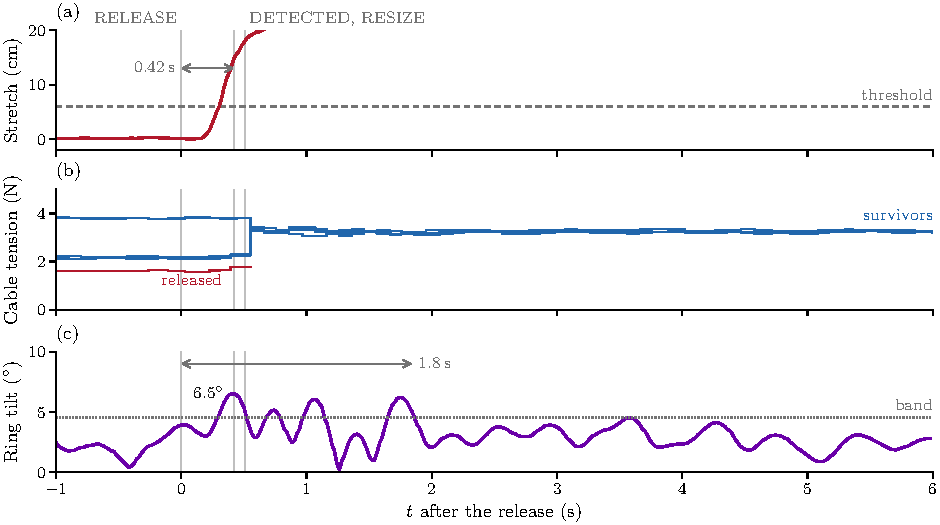
\includegraphics[width=\columnwidth]{figures/fig_release.pdf}
\caption{An unannounced release on the rig: one of four carriers (red) lets go of its plate in hover. The planner
detects the loose cable from its stretch, resizes to the three survivors (blue), and the ring's tilt (black) returns
to its band.}
\label{fig:release}
\end{figure}

\begin{table}[t]
\centering
\footnotesize
\setlength{\tabcolsep}{3pt}
\caption{Reaction to a lost carrier, four carriers in hover. Times from the release (or the command). Rig: 0.55\,m
rods; twin: 1\,m cables.}
\label{tab:release}
\begin{tabular}{lcccc}
\toprule
 & Detected & Resized & Tilt peak & Back in band \\
Case & (s) & (s) & ($^\circ$) & (s) \\
\midrule
Rig, release (Fig.~\ref{fig:release}) & 0.42 & 0.51 & 6.5 & 1.8 \\
Rig, all three releases & 0.33--0.42 & \placeholder{to measure} & 6.5--17.8 & 1.8--3.8 \\
Rig, announced detach & -- & 0 & 15.4 & 1.95 \\
Twin, release & -- & 0.37 & 5.9 & 3.4 \\
\bottomrule
\end{tabular}
\end{table}

\paragraph{A departed carrier rejoins (twin)}
A released carrier is not landed: it holds a staging point beyond its own plate and, on the operator's command,
flies back, is re-attached and is folded into the team (Section~\ref{sec:rejoin}). This is a twin result only, since
the twin's joint welds the cable wherever its end lies, while the rig's magnet catches only on contact. A rejoin is
scored in stages, each against a bar frozen before the runs: the cable's end on its plate within 30\,s; the joint
attached within 0.5\,s of that; then the fold-in, with the ring's tilt at most 5$^\circ$ from the weld to 15\,s
after it, the end within 2\,cm of its plate through the 10\,s blend, and the rejoiner's planned pull at the blend's end
within 10\,\% of its share. Table~\ref{tab:rejoin} gives the results onto a square (four carriers back from three) and
onto a T (three back from an opposite pair); Fig.~\ref{fig:rejoin} shows one rejoin onto the T.

Every rejoin welded within 1.5\,cm of its plate point, and 10 of the 11 fold-ins tilted the ring by
1.3--3.4$^\circ$. With a steady torque leaning the T's pair about 3$^\circ$, the rejoin passed 3 of 4 runs: in one run leaning toward the
rejoin plate the ring tipped to 5.28$^\circ$ for 0.19\,s, missing the bar by 0.28$^\circ$. There the rejoiner's
height reference, held at or below its weld height through the blend to stop its rigid link lifting the T's free side,
dipped 1.1\,cm at the fold-in. The hold patches a twin artefact, a rigid link, which the rig's slack tethers do not
share. Two neighbouring checks also passed: a LAND during the rejoin's descent sends the rejoiner up, out and down
alone, 1.245\,m from the ring's centre (bar 1.2\,m), and a carrier staged through a figure-eight lap of the T stays
inside the position limit, with its attach command refused while the path moves.

\begin{table}[t]
\centering
\footnotesize
\setlength{\tabcolsep}{2.2pt}
\caption{A departed carrier rejoins its own plate (twin, hover, 1\,m cables), final code tree. Bars, frozen before
the runs, in brackets. Leaning: a steady torque leans the T's pair about 3$^\circ$. Ranges over $n$ runs.}
\label{tab:rejoin}
\begin{tabular}{lccccc}
\toprule
 & & On plate & Weld & Fold-in & End from \\
Rejoin & $n$ & after (s) & after (s) & tilt ($^\circ$) & plate (cm) \\
 & & [30] & [0.5] & [5] & [2] \\
\midrule
Square & 4 & 23.9--24.9 & 0.029--0.036 & 1.27--1.55 & 1.3--1.6 \\
T & 3 & 16.6--17.7 & 0.012--0.021 & 1.45--3.02 & 1.3--1.5 \\
T, leaning toward & 2 & 15.6--16.5 & 0.015--0.018 & 3.12--\textbf{5.28} & 1.3--1.5 \\
T, leaning away & 2 & 17.7--18.6 & 0.015--0.018 & 2.91--3.37 & 1.4--1.5 \\
\bottomrule
\end{tabular}
\end{table}

\begin{figure}[t]
\centering
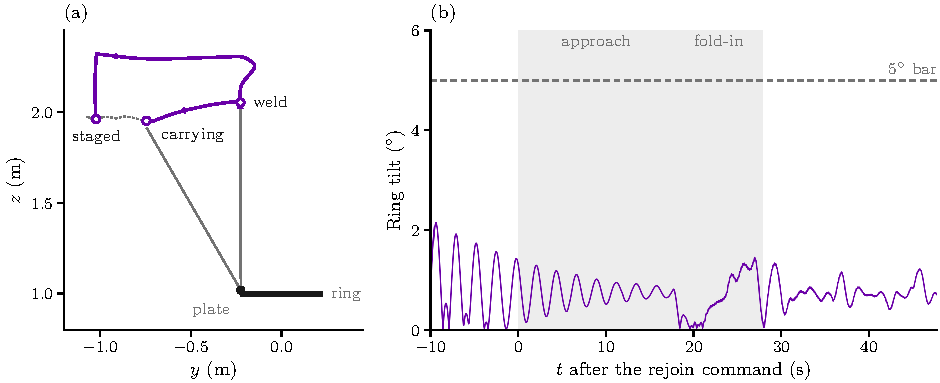
\includegraphics[width=\columnwidth]{figures/fig_rejoin.pdf}
\caption{A carrier released from the T flies back to its own plate in the twin, re-welds 17.8\,s after the rejoin
command and folds back in. (a) The rejoiner's path, side view, with its cable at the weld and folded in; (b) the
ring's tilt, peaking at 1.45$^\circ$ in the fold-in, against the 5$^\circ$ bar.}
\label{fig:rejoin}
\end{figure}

\paragraph{Eight to four and back (twin)}
Release and rejoin compose into a chain. Eight carriers at 45$^\circ$ on 1\,m cables lift a 0.9\,kg ring of radius
0.5\,m from the floor; every other carrier is released unannounced, one at a time and 15\,s apart, down to a square of four,
and the four freed carriers then rejoin one at a time back to eight (Fig.~\ref{fig:s_chain}). In both claim runs, at five
solver iterations per tick, no drop or abort fired; each release raised the ring's tilt by at most 2.9$^\circ$ with the
planner resized within 0.4\,s, and each rejoin's planner grew within 16.2--19.4\,s of its start. Back at eight, scored from
2\,s after the last rejoin's blend ends, the ring's tilt held its bar (0.95--0.99$^\circ$) but its position error, 6.4\,mm
(rms) in both runs, missed its bar of 5.7\,mm: the last fold-in leaves the ring 36\,mm off, and it returns over about 5\,s.
The world runs at about a quarter of real time here, so these runs are about the plan and the physics, not about timing
(Section~\ref{sec:res_scale}).

\begin{figure}[t]
\centering
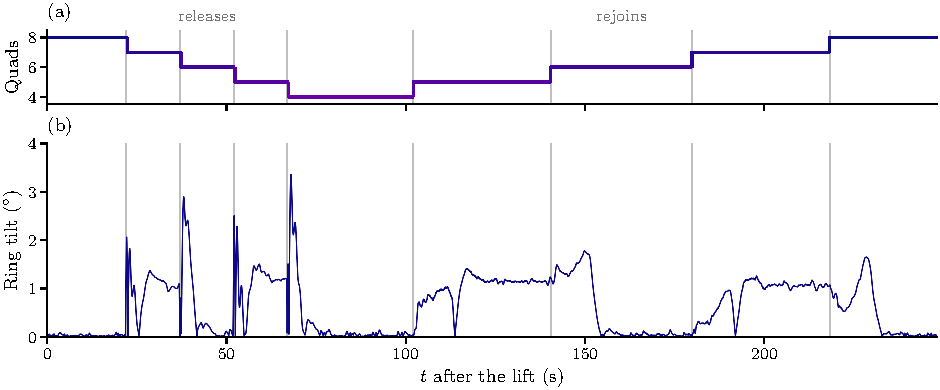
\includegraphics[width=\columnwidth]{figures/fig_s_chain.pdf}
\caption{Eight carriers take the 0.9\,kg, 0.5\,m ring through four unannounced releases down to four and four
rejoins back to eight (twin, not real time; an earlier exploratory run at one iteration a tick, the claim runs at
five described in the text). (a) The team size the planner flies; (b) the ring's tilt, peaking at 3.35$^\circ$.}
\label{fig:s_chain}
\end{figure}

\paragraph{A newcomer attaches on the rig}
\placeholder{The rig attach of a newcomer on 1\,m cables (three carriers to four with the basket): flies 29 Oct.}

